%%%%%%%%%Template for reFUEL presentations%%%%%%%%%

%%%%%%%%%Version 0.1%%%%%%%%%
%%%%%%%%%Author: Johannes Schmidt%%%%%%%%%

\documentclass[color=usenames,dvipsnames]{beamer}
% aspectratio=169

\mode<presentation> {

    \usetheme{Madrid}
    \usepackage{tikz}
    \usepackage{booktabs}
    \usepackage{qrcode}

    % Thin fonts
    \usepackage{cmbright}
    \usepackage[T1]{fontenc}

    \usetikzlibrary{shapes.geometric, arrows}

    %%%Definition of ERC colors
    \definecolor{ERC1}{HTML}{C72321}
    \definecolor{ERC2}{HTML}{861719}
    \definecolor{ERC3}{HTML}{FBD7A9}
    \definecolor{ERC4}{HTML}{BA9F7C}
    \definecolor{ERC5}{HTML}{7A6952}
    \definecolor{ERC6}{HTML}{6E9B9E}
    \definecolor{ERC7}{HTML}{0D8085}
    \definecolor{ERC8}{HTML}{19484C}
    \definecolor{ERC9}{HTML}{F0C320}
    \definecolor{ERC10}{HTML}{AF8F19}

    %%%Definition of colors for graph elements
    \tikzstyle{startstop} = [rectangle, rounded corners, minimum width=3cm, minimum height=1cm,text centered, draw=black, fill=ERC8]
    \tikzstyle{io} = [trapezium, trapezium left angle=70, trapezium right angle=110, minimum width=3cm, minimum height=1cm, text centered, draw=black, fill=ERC7]
    \tikzstyle{process} = [rectangle, minimum width=3cm, minimum height=1cm, text centered, draw=black, fill=ERC9]
    \tikzstyle{decision} = [diamond, minimum width=3cm, minimum height=1cm, text centered, draw=black, fill=ERC10]
    \tikzstyle{arrow} = [thick,->,>=stealth]

    %%%%Definition of palette
    \setbeamercolor{palette primary}{bg=ERC1,fg=white}
    \setbeamercolor{palette secondary}{bg=ERC2,fg=white}
    \setbeamercolor{palette tertiary}{bg=ERC3,fg=white}
    \setbeamercolor{palette quaternary}{bg=ERC4,fg=white}
    \setbeamercolor{structure}{fg=ERC5} % itemize, enumerate, etc
    \setbeamercolor{section in toc}{fg=ERC6} % TOC sections

    %gets rid of bottom navigation bars
    \setbeamertemplate{footline}[frame number]{}

    %gets rid of bottom navigation symbols
    \setbeamertemplate{navigation symbols}{}

    %gets rid of footer
    %will override 'frame number' instruction above
    %comment out to revert to previous/default definitions
    \setbeamertemplate{footline}{}

    \useoutertheme{infolines}
}

\definecolor{dark_grey}{gray}{0.5}

\usefonttheme{default}

\setbeamertemplate{navigation symbols}{}
\setbeamertemplate{blocks}[rounded][shadow=false]
\setbeamertemplate{frametitle}[default][center]
\setbeamertemplate{itemize items}[default]
\setbeamertemplate{enumerate items}[default]
\setbeamertemplate{title page}[default][colsep=-4bp,rounded=true]
\setbeamertemplate{footline}[frame number]

\newcommand{\F}{\mathbb{F}}


\title{The potential for re-powering wind turbines: reducing turbines, increasing output}
\author{\small{Peter Regner\inst{1}, Katharina Gruber\inst{1}, Johannes Schmidt\inst{1}, Claude Kl\"ockl\inst{1}}}
\institute{
    \inst{1}Institute for Sustainable Economic Development,\\
    University of Natural Resources and Life Sciences, Vienna
}
\date{2019-10-20, Vienna, INFORMS 2019}

\begin{document}
    %%%%Title Page
    {
        \usebackgroundtemplate{
            \begin{picture}(320,315)
            \hspace{6.9cm}
              
\includegraphics[width=0.7\linewidth]{refuel_logo_with_text.png}
            \end{picture}
        }

        \begin{frame}[plain]
          \maketitle
          \vspace{1.7cm}
          
\includegraphics[height=0.7cm]{creative-commons-by.pdf}
          \hspace{3.05cm}
\includegraphics[height=1.7cm]{boku-logo.pdf}\\
        \end{frame}
    }

    \begin{frame}{Introduction}
        \begin{itemize}
            \item Low carbon energy systems: land usage is a critical factor \pause
            \item \textbf{repowering} = replacing power plants with newer ones,
                which have a higher rated \textbf{capacity} or more
                \textbf{efficiency}\pause
            \item How much power generation gain can be expected in the US with
                newer wind turbine models? \pause How many wind turbines will be installed?
        \end{itemize}
    \end{frame}

    \begin{frame}{Data}
        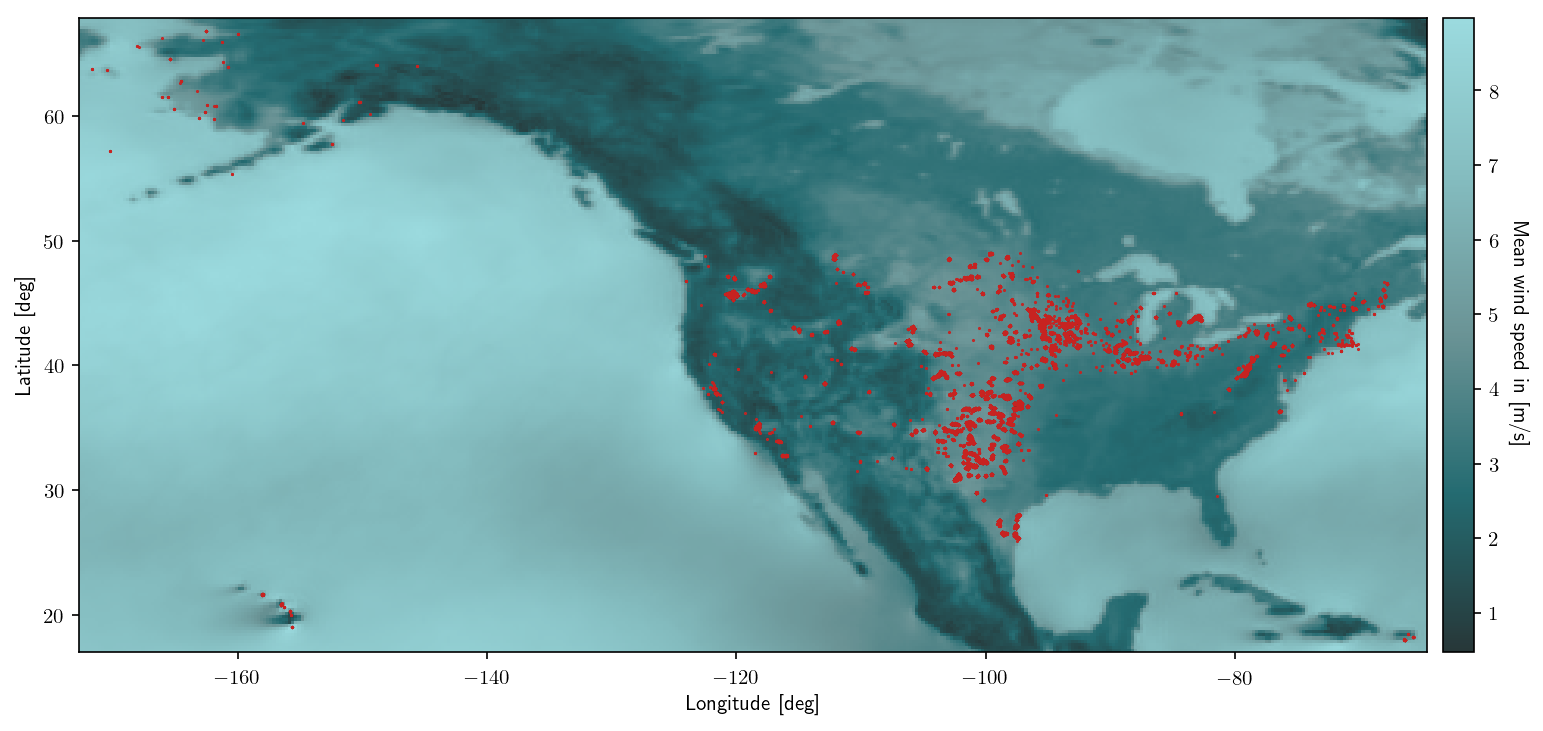
\includegraphics[width=\textwidth]{../../figures/mean_wind_speed_and_turbines.png}
    \end{frame}

    \begin{frame}{Data}
        \begin{itemize}
            \item \textbf{ERA5}: wind speed data, hourly (2001 - 2018),
                0.25$^\circ$ spatial resolution\pause
            \item \textbf{United States Wind Turbine Database (USWTDB)}:
                58,184 turbines including location, model name, rated capacity,
                rotor diameter, ...\pause
            \item Time series of \textbf{wind power net generation} provided by
                the U.S. Energy Information Administration (EIA) via the
                Electricity data browser: time series, monthly total power
                generation (2001 - 2018)\pause
            \item Data sheets for turbine models:
                \textbf{rotor diameter}, \textbf{power curve}
        \end{itemize}
    \end{frame}

    \begin{frame}{Turbine models}
        \begin{center}
            \begin{tabular}{| l | c | c | l }
                \hline
                \bfseries{Model name} & \bfseries{Rated capacity} & \bfseries{Rotor diameter}\\
                \hline
                GE-1.5 77 & 1.5 MW & 77 m\\
                \hline
                Senvion 3.4M114 & 3.4 MW & 114 m\\
                \hline
                Enercon E-138 EP3 & 3.5 MW & 138 m\\
                \hline
                Senvion 4.2M140 & 4.2 MW & 140 m\\
                \hline
                Enercon E-126 & 7.58MW & 127 m\\
                \hline
            \end{tabular}
        \end{center}

        \bigskip

        GE-1.5 77 is the most frequent model in the U.S. (14.7\% of all turbines).

    \end{frame}

    \begin{frame}{Power curves}
        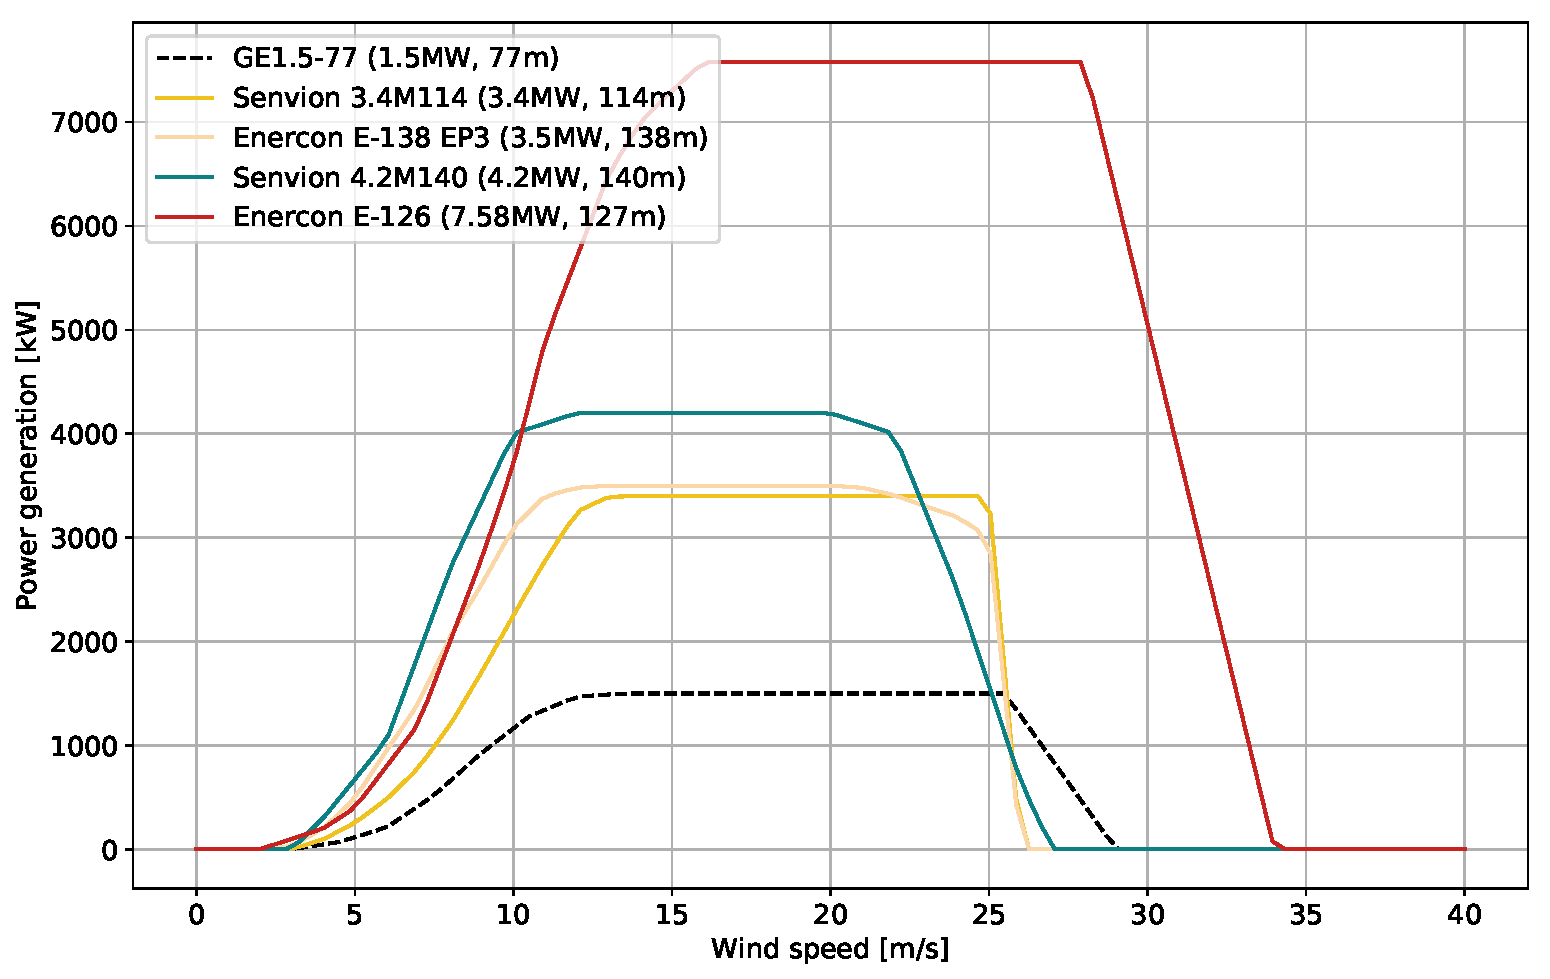
\includegraphics[width=\textwidth]{../../figures/power_curves.pdf}
    \end{frame}

    \begin{frame}{Simulation of power generation}
        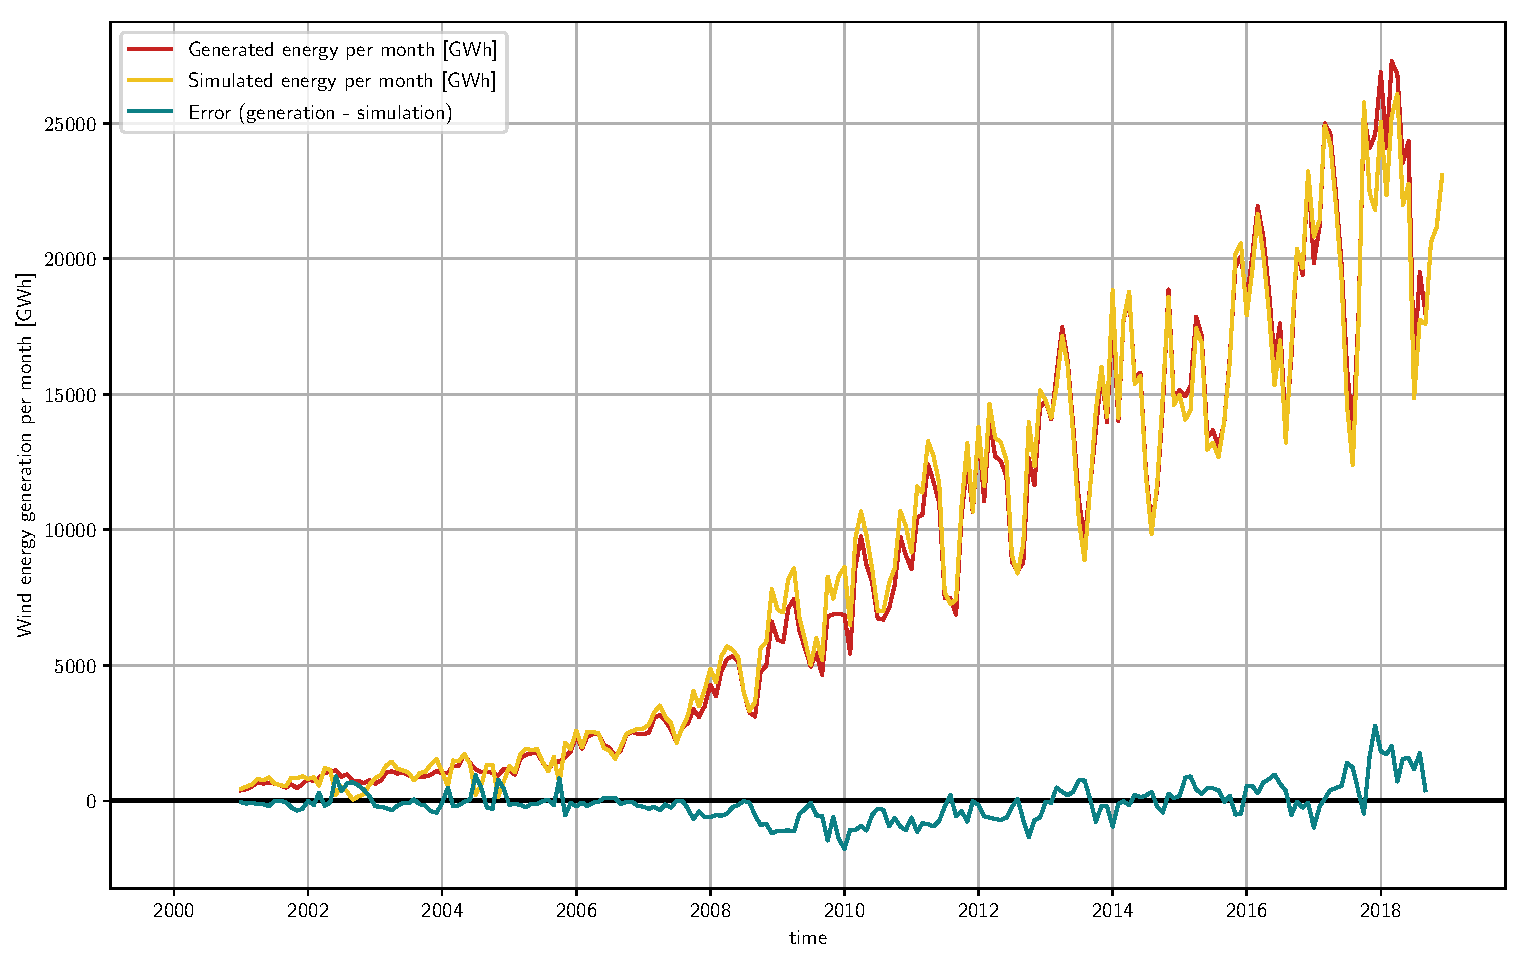
\includegraphics[width=\textwidth]{../../figures/simulated-energy_time-series.pdf}
    \end{frame}

    %\begin{frame}{Historical development of wind turbine characteristics}
        %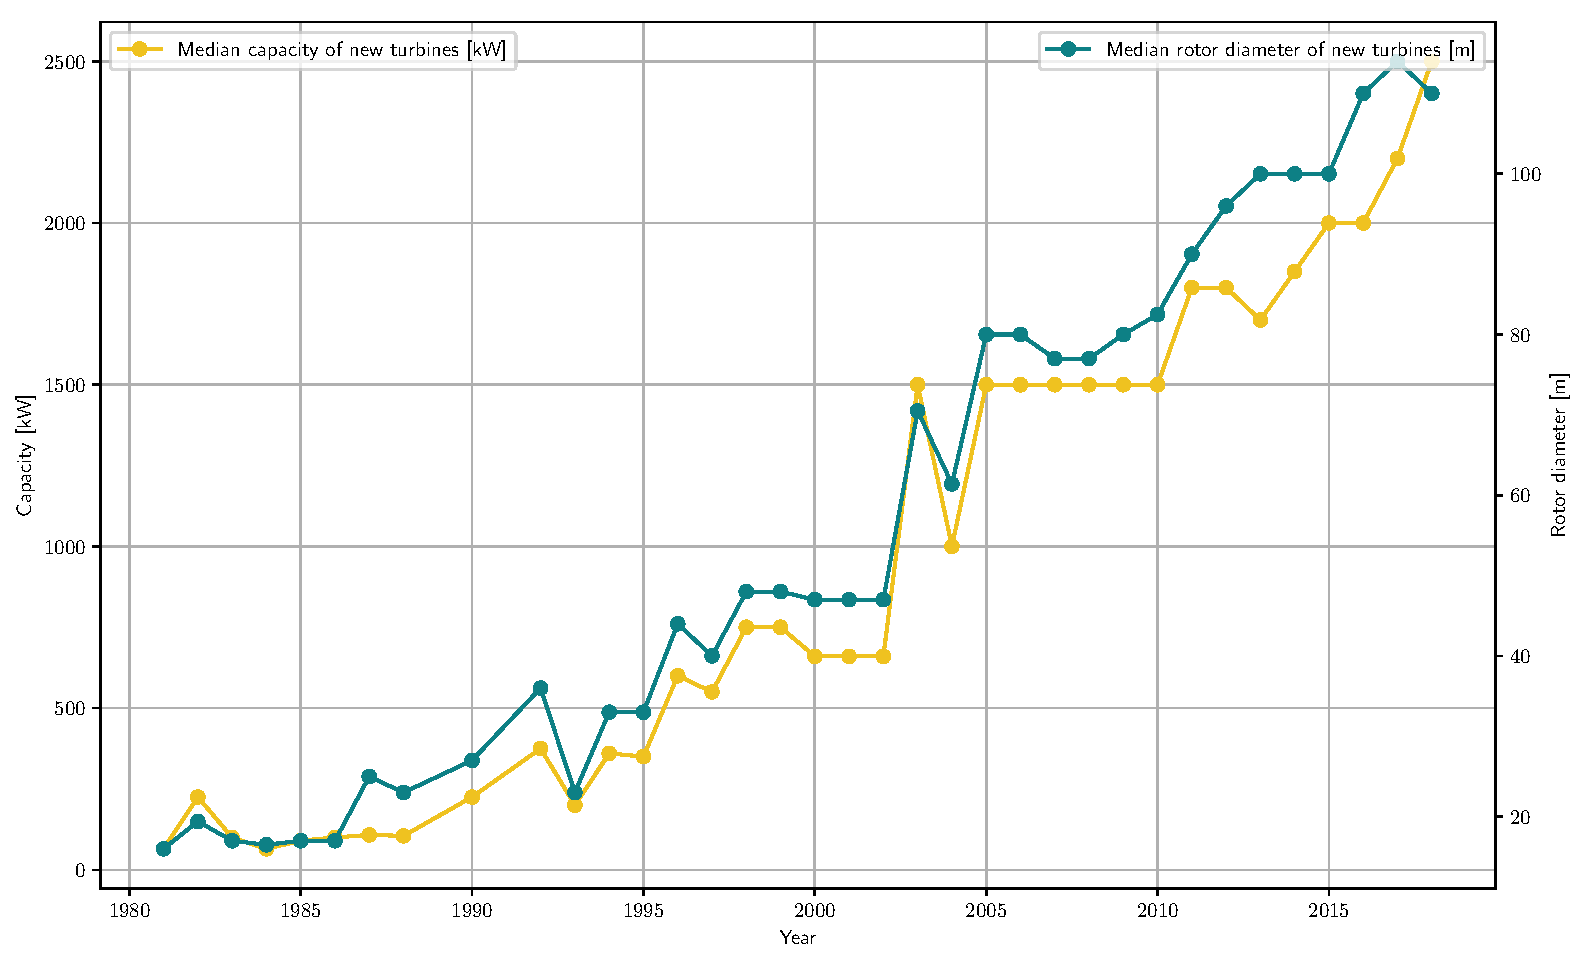
\includegraphics[width=\textwidth]{../../figures/history_turbines.pdf}
    %\end{frame}

    \begin{frame}{Maximum power generation with different turbines}
        \textbf{Optimization problem}:\\
        \bigskip
        Existing turbines are replaced by newer ones at the location of the old
        turbines, such that:\\
        \begin{itemize}
            \item objective function: total power generation is maximized
            \item constraints: distance between turbines is not below a threshold\pause ,
                which depends on the direction relative to the prevailing wind direction
                at the location
        \end{itemize}
    \end{frame}

    %\begin{frame}{Overview of calculations}
    %    %- data flow diagram
    %    %    - linear interpolation
    %\end{frame}

    %- error measures of simulation
    %    --> correlation
    %    --> rmse
    %
    %- weibull

    \begin{frame}{Optimal locations for new wind turbines}
        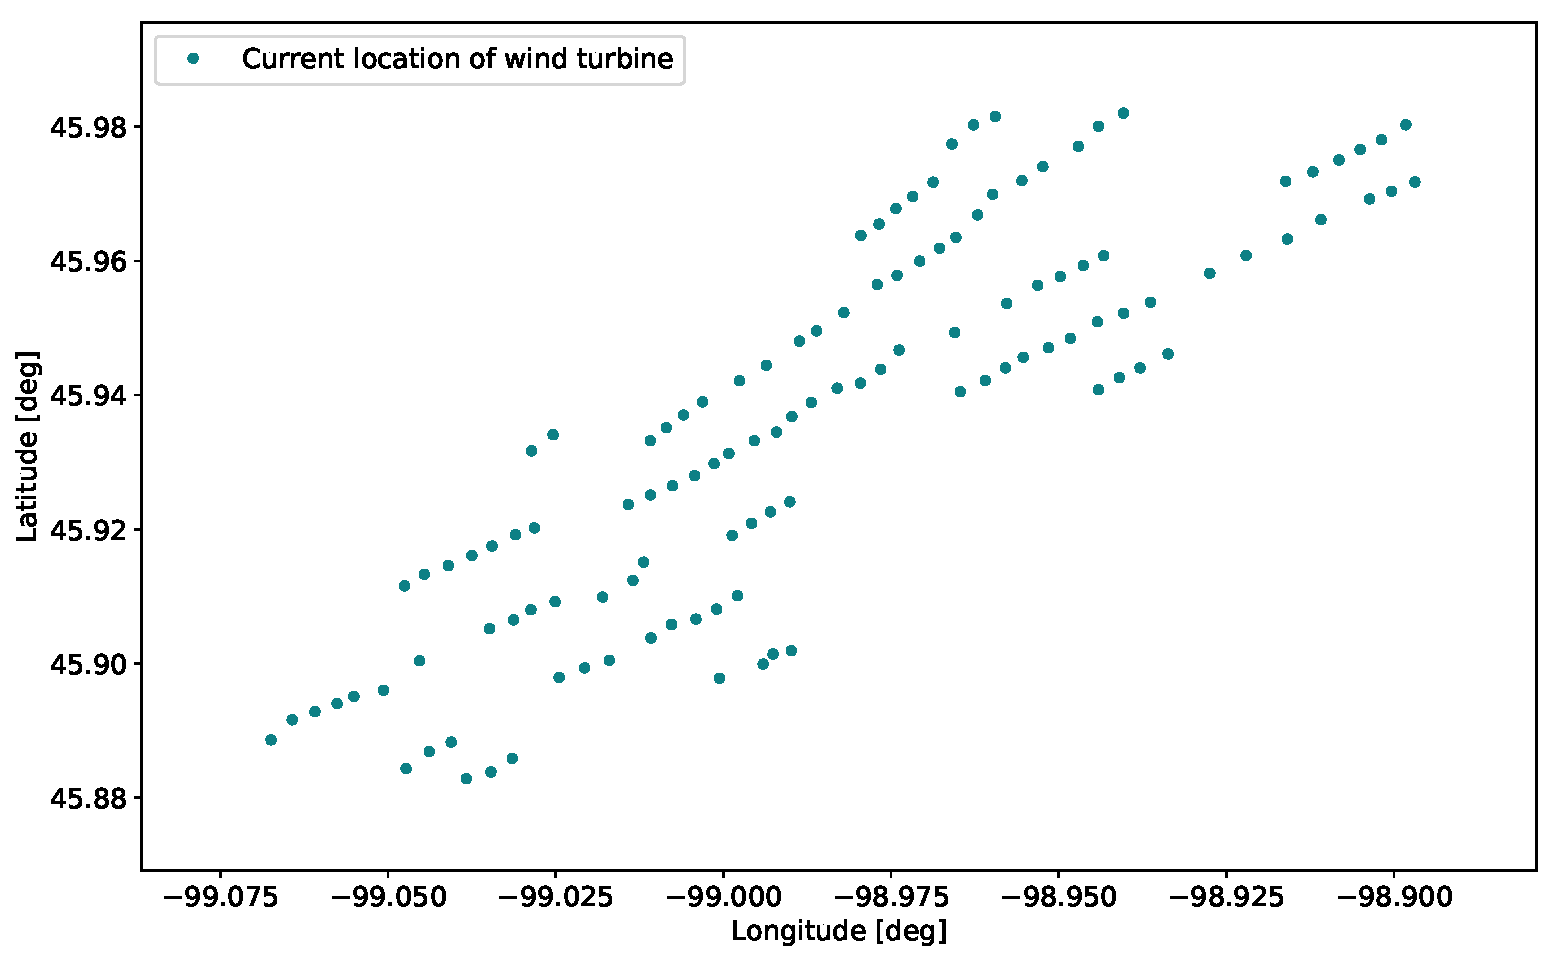
\includegraphics[width=\textwidth]{../../figures/optimized_cluster-0.pdf}
    \end{frame}

    \begin{frame}{Optimal locations for new wind turbines}
        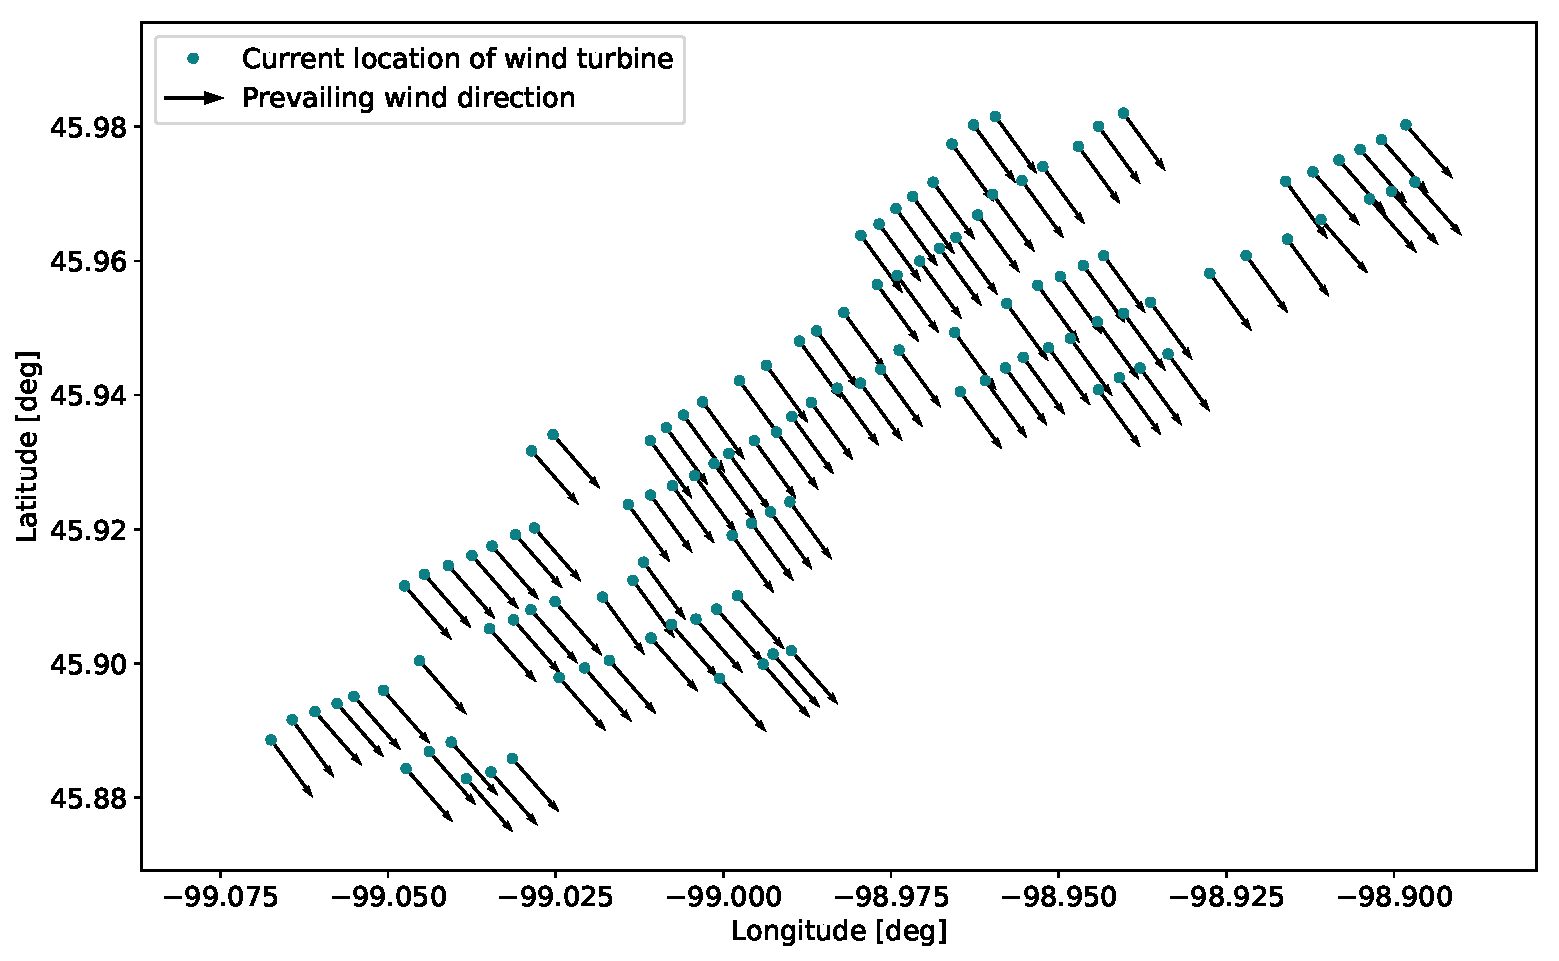
\includegraphics[width=\textwidth]{../../figures/optimized_cluster-1.pdf}
    \end{frame}

    \begin{frame}{Optimal locations for new wind turbines}
        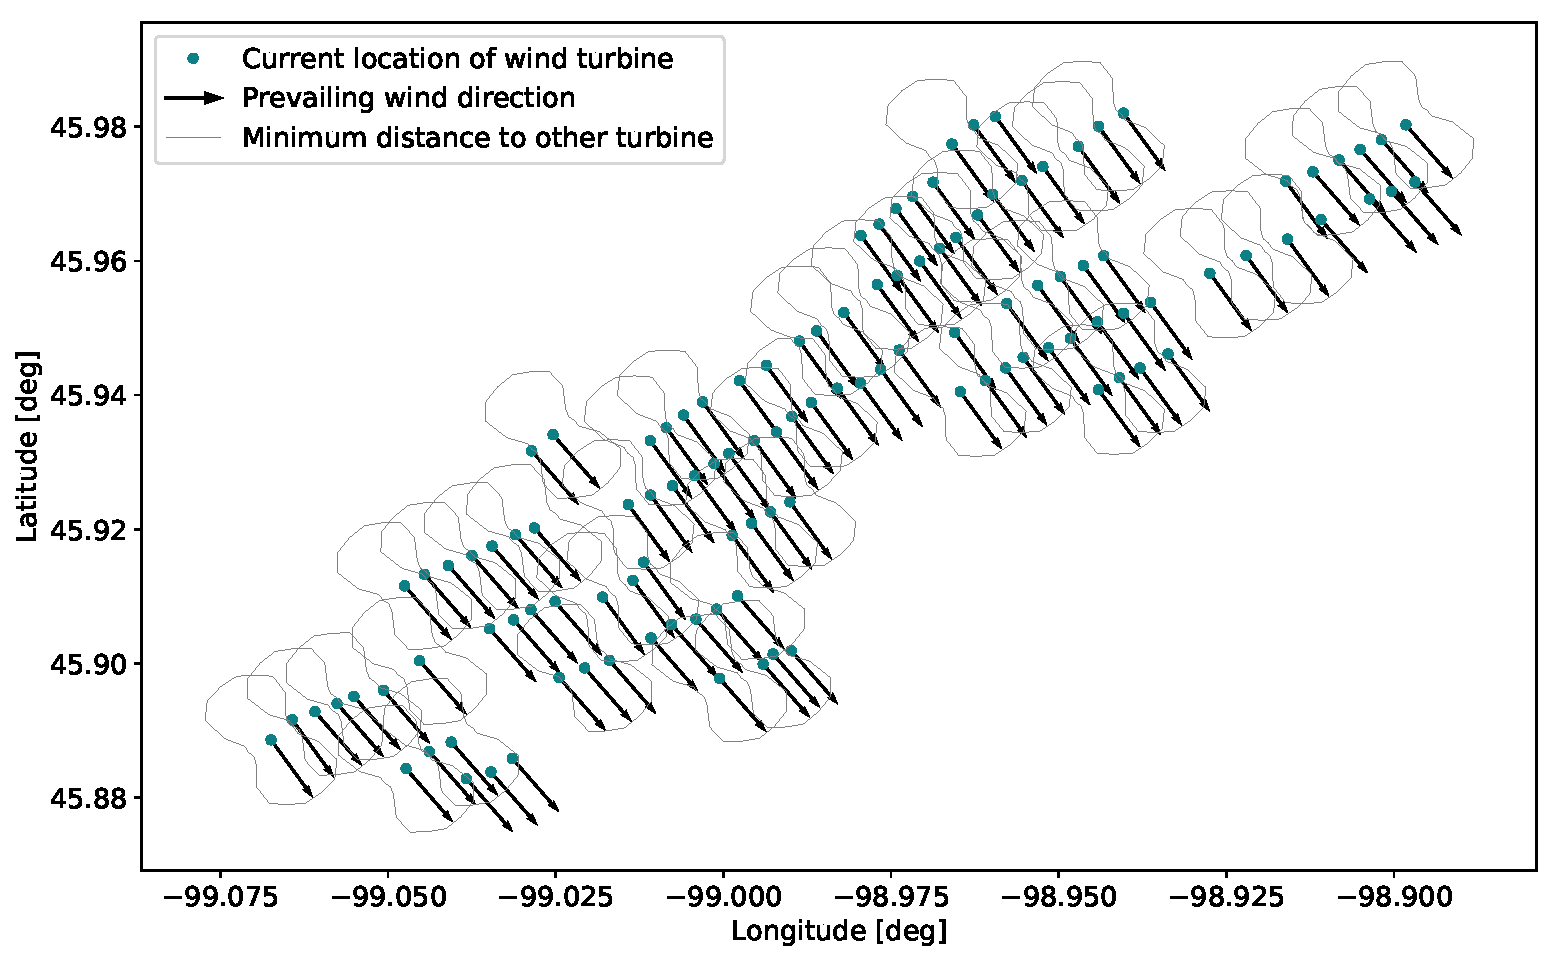
\includegraphics[width=\textwidth]{../../figures/optimized_cluster-2.pdf}
    \end{frame}

    \begin{frame}{Optimal locations for new wind turbines}
        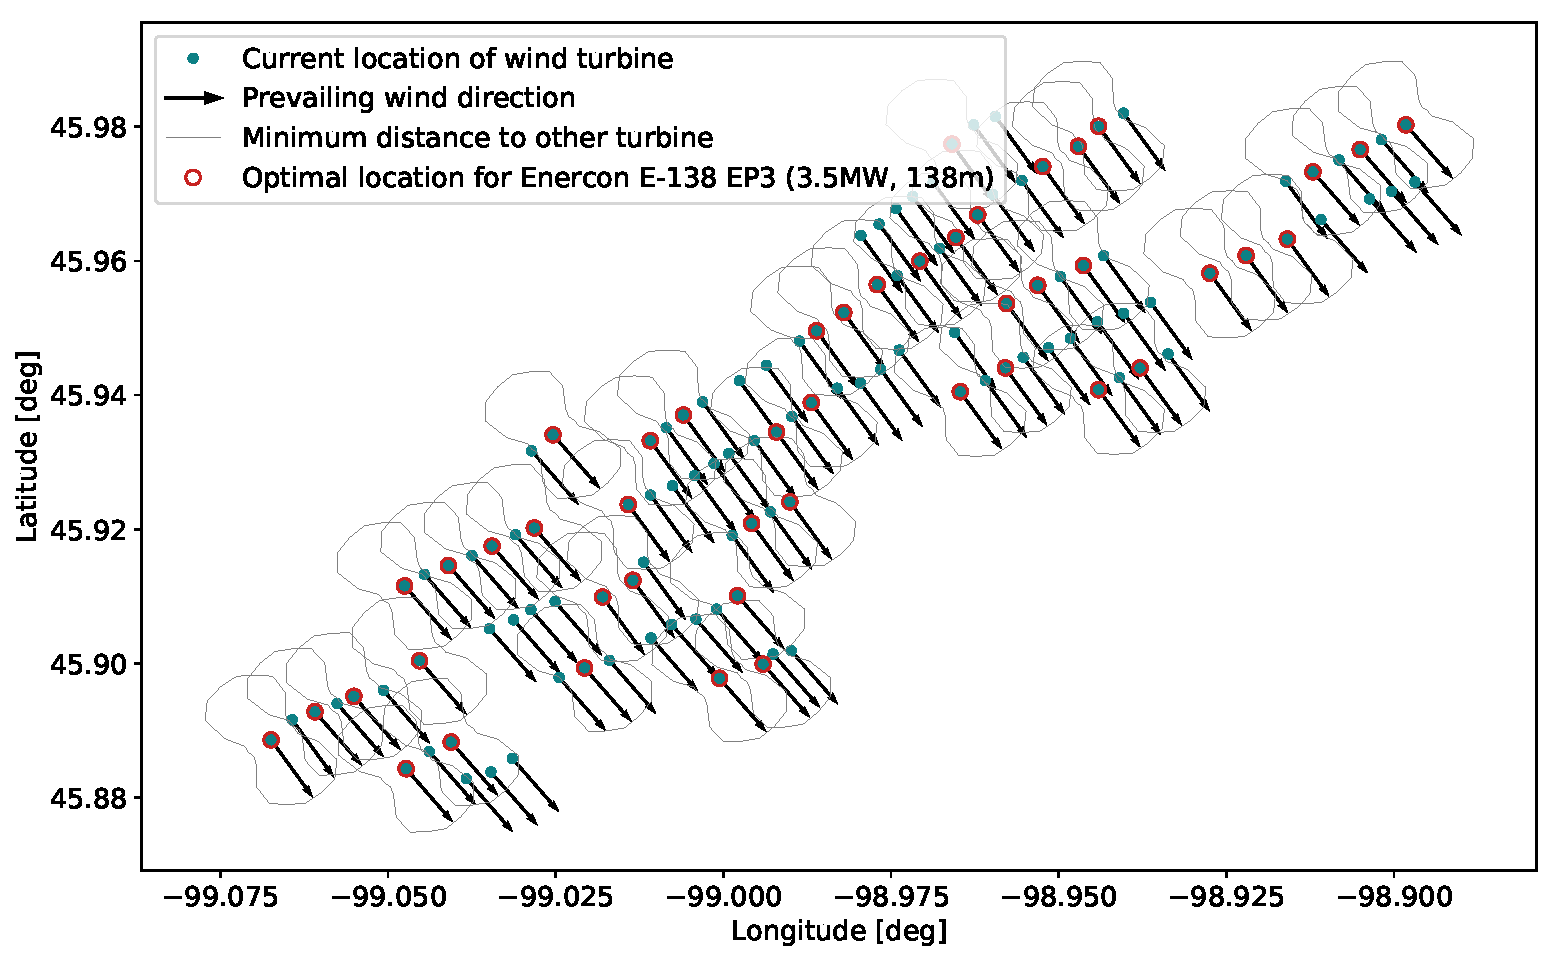
\includegraphics[width=\textwidth]{../../figures/optimized_cluster-3.pdf}
    \end{frame}

    \begin{frame}{Minimum distances between turbine locations}
        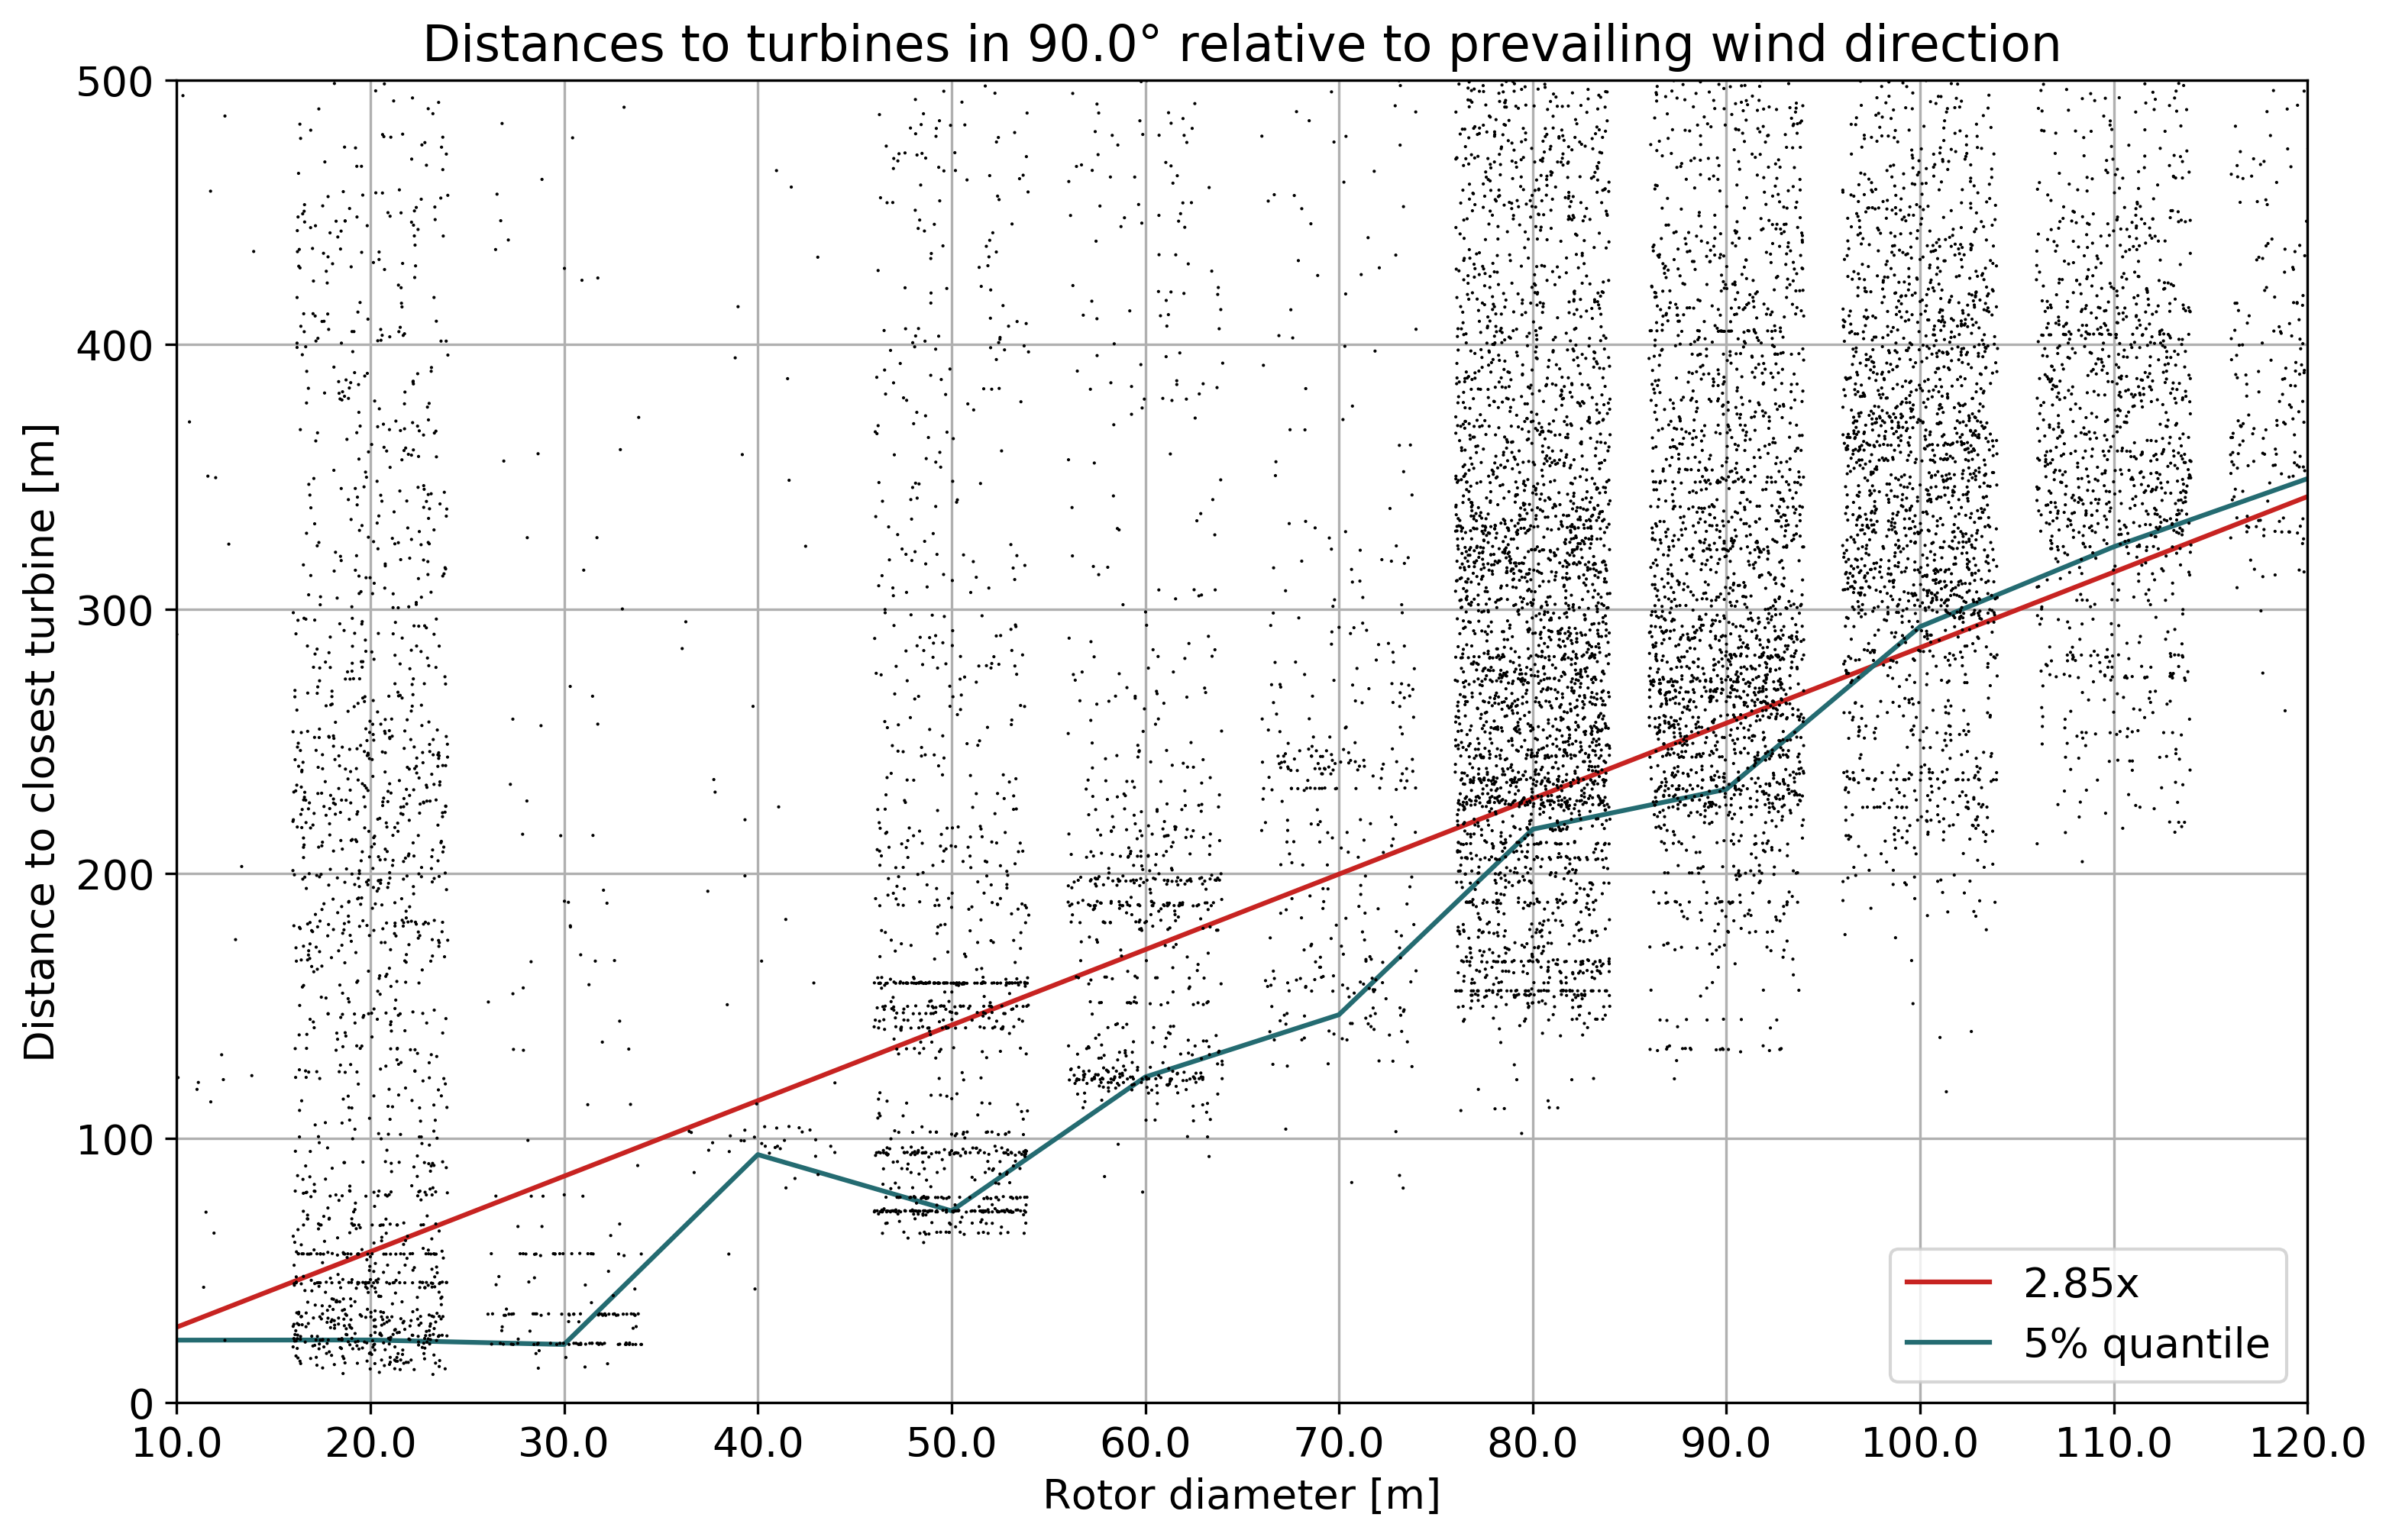
\includegraphics[width=\textwidth]{../../figures/distances_between_turbines.png}
    \end{frame}

    \begin{frame}{Repowering potential: power generation}
        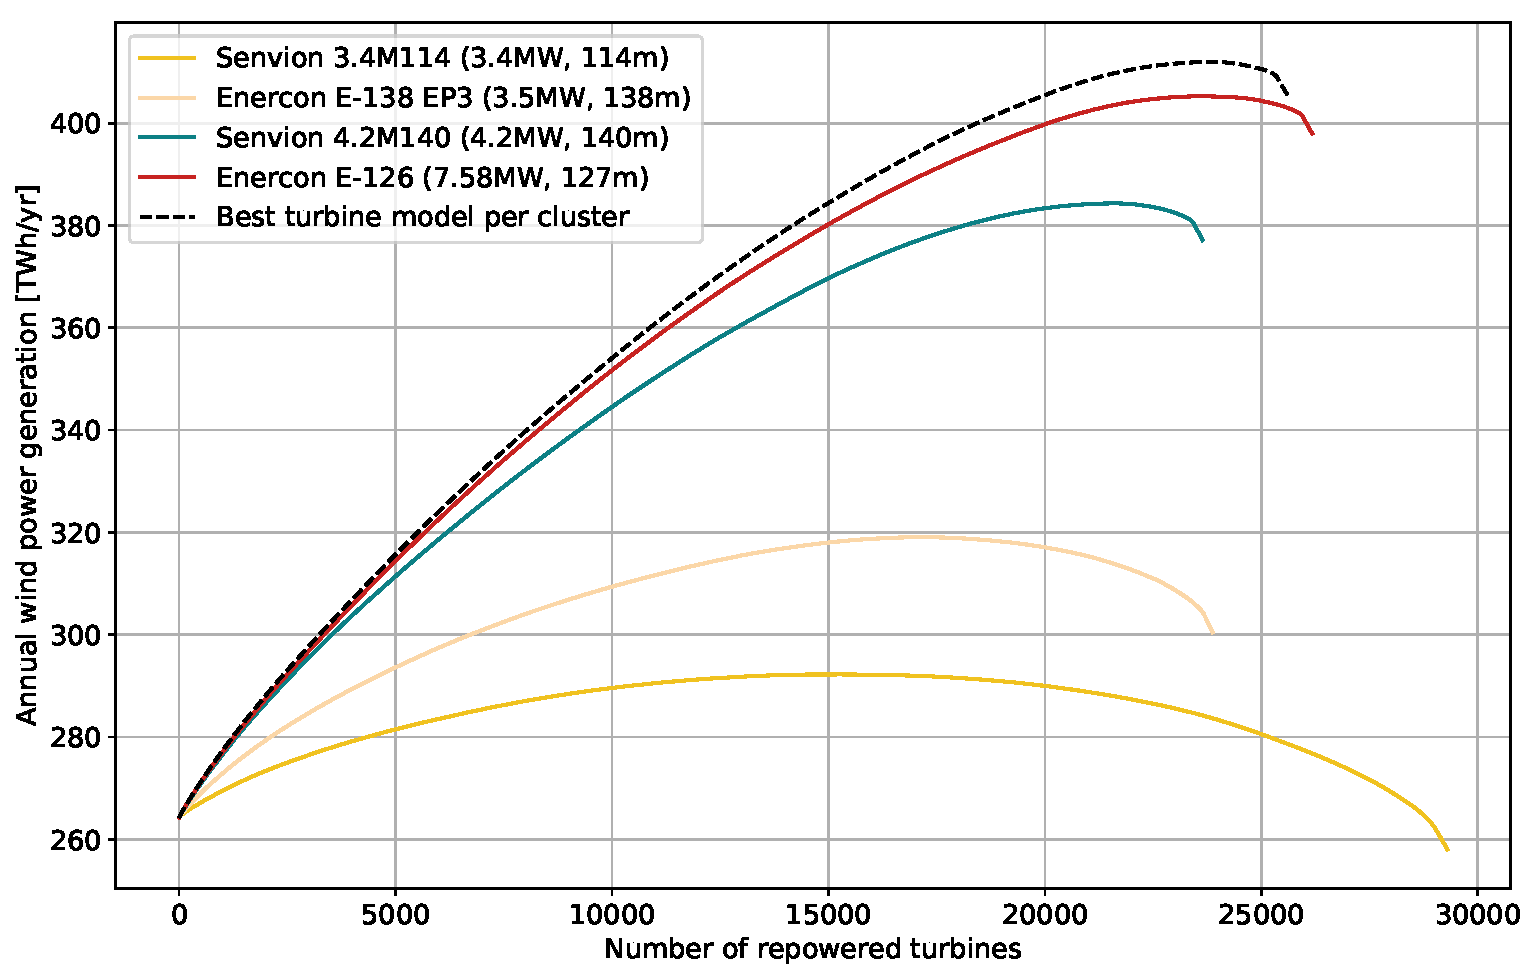
\includegraphics[width=\textwidth]{../../figures/repower_potential-direction-dependent_power_generation.pdf}
    \end{frame}

    \begin{frame}{Repowering potential: number of turbines}
        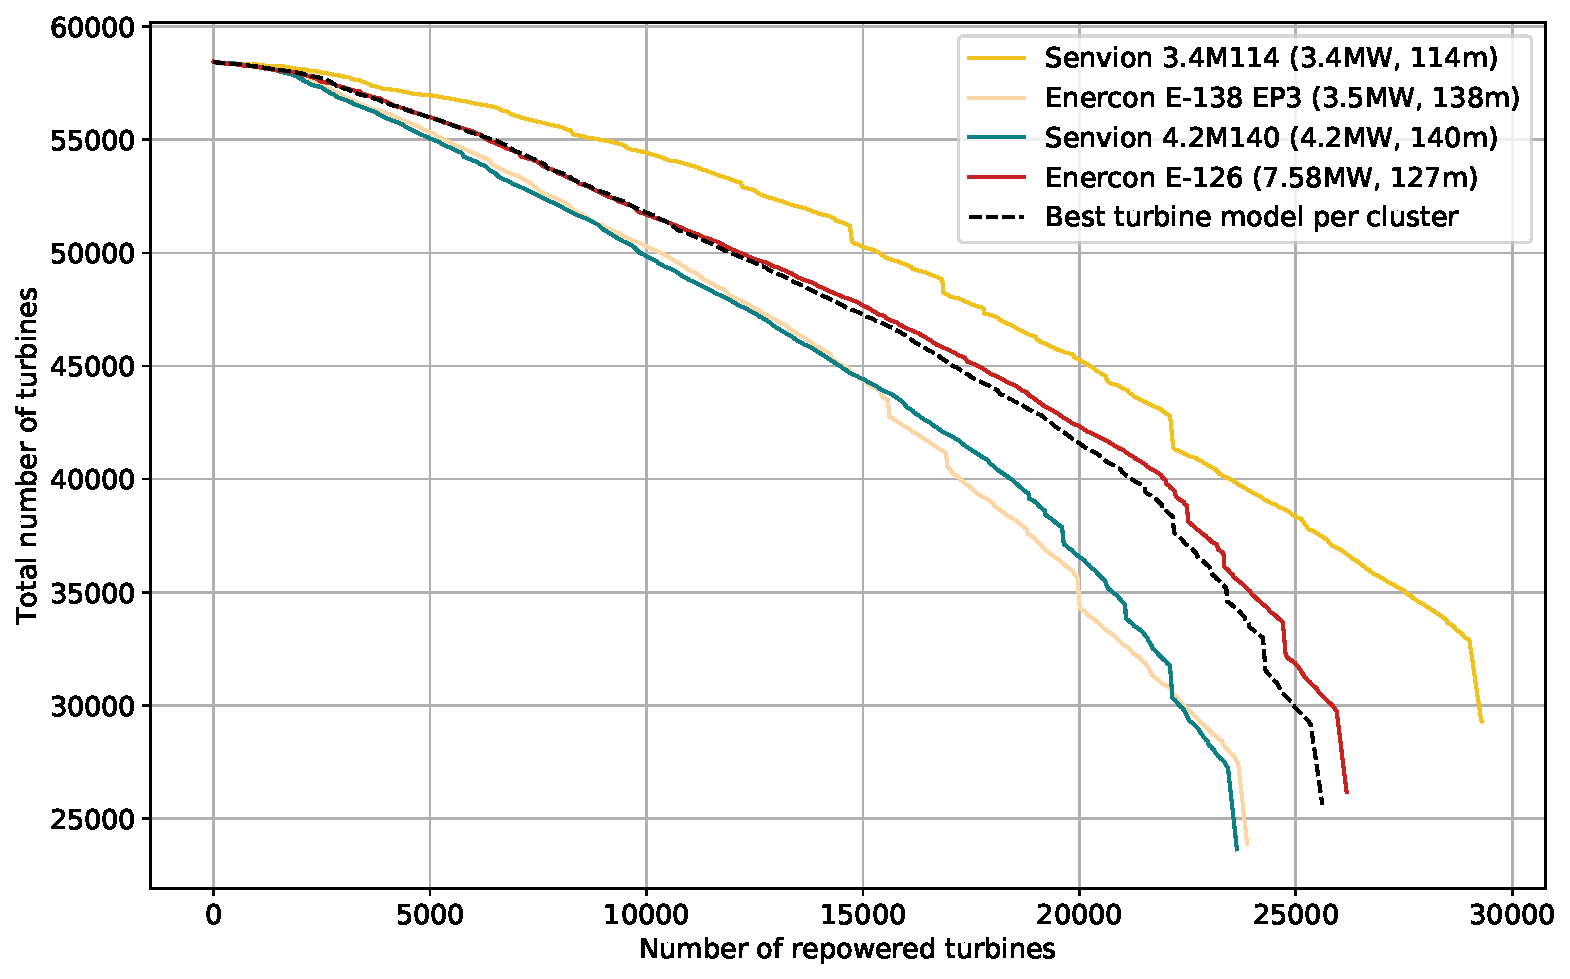
\includegraphics[width=\textwidth]{../../figures/repower_potential-direction-dependent_num_turbines.pdf}
    \end{frame}

    \begin{frame}{Conclusions}
        Conclusions:\\
        \begin{itemize}
            \item repowering less than half of the existing turbines, roughly increases the
                power generation output by 50\%\pause
            \item repowering leads to a significant drop of total number of
                turbines installed\pause
            \item minimum distances between wind turbines can be estimated by a
                linear model using the rotor diameter\pause
        \end{itemize}
    \end{frame}

    %%%Last Frame
    {
    \usebackgroundtemplate{
        \begin{picture}(200,305)
        \hspace{7.7cm}
          
\includegraphics[width=0.6\linewidth]{refuel_logo_with_text.png}
        \end{picture}
    }
    \begin{frame}[plain]
        \frametitle{Thank you!}
        \vspace{1.5cm}
        https://refuel.world/\\
        peter.regner@boku.ac.at\\
        http://bit.ly/wind-repower-us\\

        \vspace{0.6cm}
        \qrcode[height=1.4cm]{http://bit.ly/wind-repower-us}\\

        \vspace{1.95cm}
        
\includegraphics[height=0.7cm]{creative-commons-by.pdf}\\
        \smallskip
        \tiny{We gratefully acknowledge support from the European\\
        Research Council (“reFUEL” ERC-2017-STG 758149).}
    \end{frame}
    }

\end{document}
